\documentclass[tikz]{standalone}
\usepackage{pgffor}

\begin{document}
    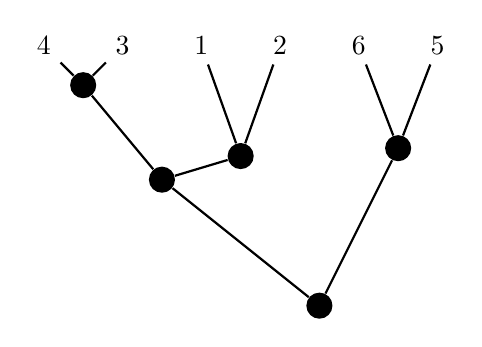
\begin{tikzpicture}
        %for 1:
        \iffalse
        \foreach \x/\y/\n/\l in {1/0/a1/1,2/0/a2/2,3/0/a3/3,4/0/a4/4,5/0/a5/5,6/0/a6/6}{
            \node[] (\n) at (\x,\y) {\l};
        }
        \foreach \x/\y/\n/\l in {0.5/1.2/n1/,2.5/0.8/n2/,4.5/1.5/n3/,1.5/2/n12/,3.5/3/r/}{
            \node[
                %shape = circle, fill = black
                ] (\n) at (1+\x,-\y) {};
            \draw[dashed] (\n) -- (1+\x,0);
        }
        \fi
        %for 2:
        \foreach \x/\y/\n/\l in {3/0/a1/1,4/0/a2/2,2/0/a3/3,1/0/a4/4,6/0/a5/5,5/0/a6/6}{
            \node[] (\n) at (\x,\y) {\l};
        }

        \foreach \x/\y/\n/\l in {2.5/1.2/n1/0.2,0.5/0.8/n2/-0.3,4.5/1.5/n3/-0.2,1.5/2/n12/-0.3,3.5/3/r/0.3}{
            \iffalse
            \node[
                %shape = circle, fill = black
                draw, shape = circle, dashed
                ] (\n) at (1+\x,-\y) {};
                 \fi
            \node[
                shape = circle, fill = black
                    ] (\n) at (1+\x,-\y - \l) {};
            \iffalse
            \draw[dashed] (\n) -- (1+\x,0);
            \fi
        }
        
        \foreach \m/\n/\l in {a1/n1/,a2/n1/,a3/n2/,a4/n2/,a5/n3/,a6/n3/,n1/n12/,n2/n12/,n12/r/,n3/r/}{
            \draw[thick] (\m) -- node[right]{\l} (\n);
        }
    \end{tikzpicture}
\end{document}